%!TEX root = ../Thesis.tex
\section{Systemdesign und Herausforderungen}
Die Architektur ist im Sinne der Übersicht und Erweiterbarkeit klar in drei Teile aufgeteilt. 
Zur Datenspeicherung wird eine Aurora-Datenbank verwendet, mit welcher über eine NodeJS API von einem in 
React erstellten User Interface kommuniziert werden kann. Die Datenbank soll in der Lage sein, 
Attribut-Wert-Paare flexibel beherbergen zu können, und dabei die bestmögliche Performanz aufweisen.
\subsection{Datenbankarchitektur}
Um die Erweiterbarkeit der Anwendung zu garantieren, muss die Datenstruktur fest sein. \footnote{quelle bitte} Trotzdem muss die Datenbank aber 
in der Lage sein, flexibel unterschiedliche Attribute und Werte speichern zu können. Das soll folgende Datenstruktur erreichen:\break

\begin{figure}[H]
    \centering
    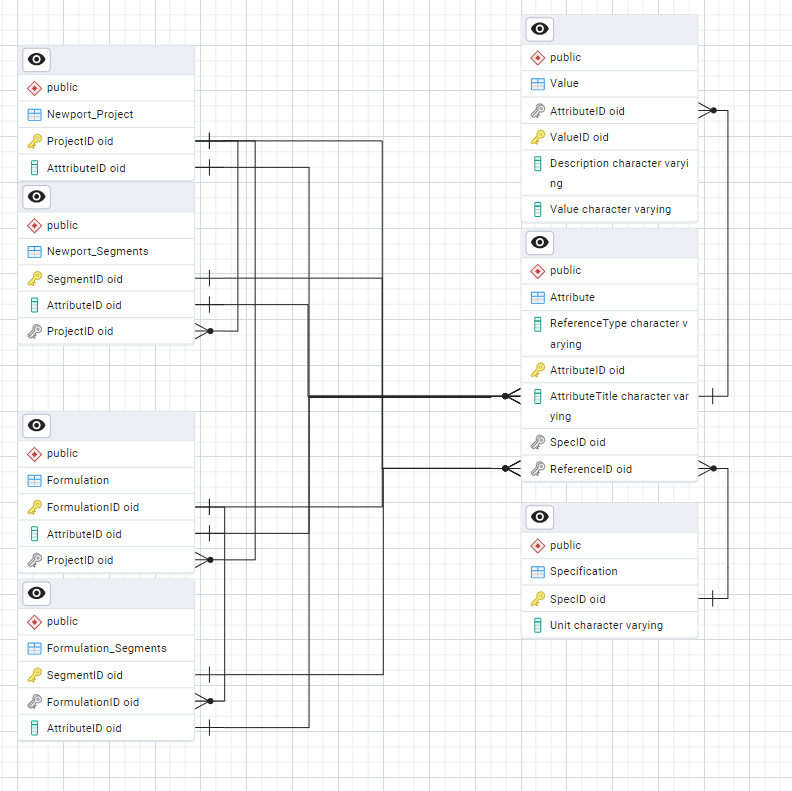
\includegraphics[width=\textwidth]{./img/datenstruktur.png} 
    \caption{Modell der Datenbank}
    \label{fig:deinbild}
\end{figure}
Die Datentruktur lässt sich in drei wesentliche Schichten aufteilen: An erster Stelle stehen die festen Datenobjekte, 
welche gleichlautend aus der bestehenden Infrastruktur übernommen werden. Diese Schicht bildet das Bindeglied zwischen der bereits existierenden Datenlandschaft 
und der von dieser Anwendung angehängten flexiblen Daten. Darauf folgt die dynamische Attributzuordnung, die über Fremdschlüssel direkt mit der ersten Schicht verbunden ist.
Sie dient zur Verlinkung verschiedener Attribute mit ihren jeweiligen Eltern-Tabellen, speichert zusätzlich aber auch grundlegende Informationen über die Attribute ab. 
Die dritte Schicht beherbergt die Werte, und verbindet diese mit ihren zugehörigen Attributen. In dieser Schicht sind Informationen zu der Natur der Werte, aber auch zum Inhalt abgespeichert. 
Im Folgenden sollen diese drei Schichten mit ihren jeweiligen Tabellen genauer beleuchtet werden. 
\subsubsection{1. Domänenspezifische Tabellen}
\enquote{Newport\_Project} bildet das übergeordnete Forschungsprojekt und ihre zugehörigen Daten ab, wobei \enquote{Formulation} nur ein Forschungsobjekt beschreibt, welches an ein Projekt geknüpft sein kann,
aber nicht unbedingt muss: 


\begin{table}[H]
    \centering
    \caption{Newport\_Project}
    \begin{tabularx}{\textwidth}{l l l X}
        \toprule
        \textbf{Spalte} & \textbf{Datentyp} & \textbf{Schlüssel?} & \textbf{Beschreibung} \\
        \midrule
        ProjectID & Object Identifier (oid) & Primärschlüssel & Primärer Identifier für den Eintrag \\
        AttributeID & Object Identifier (oid) & Fremdschlüssel & Verweis auf zugewiesene Attribute für das jeweilige Projekt \\
        \bottomrule
    \end{tabularx}
    \source{Eigene Darstellung}
    \label{tab:newport_project}
\end{table}

\begin{table}[H]
    \centering
    \caption{Formulation}
    \begin{tabularx}{\textwidth}{l l l X}
        \toprule
        \textbf{Spalte} & \textbf{Datentyp} & \textbf{Schlüssel?} & \textbf{Beschreibung} \\
        \midrule
        FormulationID & Object Identifier (oid) & Primärschlüssel & Primärer Identifier für den Eintrag\\
        AttributeID & Object Identifier (oid) & Fremdschlüssel & Verweis auf zugewiesene Attribute für das jeweilige Projekt\\
        ProjectID & Object Identifier (oid) & Fremdschlüssel & Verweis auf ein gegebenenfalls zugewiesenes Newport-Projekt\\
        \bottomrule
    \end{tabularx}
    \source{Eigene Darstellung}
    \label{tab:formulation}
\end{table}

\begin{table}[H]
    \centering
    \caption{Newport\_Segments}
    \begin{tabularx}{\textwidth}{l l l X}
        \toprule
        \textbf{Spalte} & \textbf{Datentyp} & \textbf{Schlüssel?} & \textbf{Beschreibung} \\
        \midrule
        SegmentID & Object Identifier (oid) & Primärschlüssel & Primärer Identifier für den Eintrag\\
        AttributeID & Object Identifier (oid) & Fremdschlüssel & Verweis auf zugewiesene Attribute für das jeweilige Segment\\
        ProjectID & Object Identifier (oid) & Fremdschlüssel & Verweis auf das zugehörige Newport-Projekt\\
        \bottomrule
    \end{tabularx}
    \source{Eigene Darstellung}
    \label{tab:newport_segments}
\end{table}

\begin{table}[H]
    \centering
    \caption{Formulation\_Segments}
    \begin{tabularx}{\textwidth}{l l l X}
        \toprule
        \textbf{Spalte} & \textbf{Datentyp} & \textbf{Schlüssel?} & \textbf{Beschreibung} \\
        \midrule
        SegmentID & Object Identifier (oid) & Primärschlüssel & Primärer Identifier für den Eintrag\\
        Formulation & Object Identifier (oid) & Fremdschlüssel & Verweis auf zugewiesene Attribute für das jeweilige Segment\\
        ProjectID & Object Identifier (oid) & Fremdschlüssel & Verweis auf das zugehörige Newport-Projekt\\
        \bottomrule
    \end{tabularx}
    \source{Eigene Darstellung}
    \label{tab:formulation_segments}
\end{table}
\subsubsection{2. Attributebene}
\begin{table}[H]
    \centering
    \caption{Attribute}
    \begin{tabularx}{\textwidth}{l l l X}
        \toprule
        \textbf{Spalte} & \textbf{Datentyp} & \textbf{Schlüssel?} & \textbf{Beschreibung} \\
        \midrule
        ReferenceType & String (oid) & / & Automatisch gesetzte wörtliche Referenz auf den Owner des Attributs\\
        ReferenceID & Object Identifier (oid) & Fremdschlüssel & Direkter Verweis auf den Owner des Attributs\\
        AttributeID & Object Identifier (oid) & Primärschlüssel & Verweis auf das zugehörige Attribut\\
        AttributeTitle & String & / & Titel des Attributs\\
        SpecID & Object Identifier (oid) & Fremdschlüssel & Verweis auf die zugehörige Spezifikation\\
        \bottomrule
    \end{tabularx}
    \source{Eigene Darstellung}
    \label{tab:attribute}
\end{table}
\subsubsection{3. Werteebene und Spezifikation}
\begin{table}[H]
    \centering
    \caption{Value}
    \begin{tabularx}{\textwidth}{l l l X}
        \toprule
        \textbf{Spalte} & \textbf{Datentyp} & \textbf{Schlüssel?} & \textbf{Beschreibung} \\
        \midrule
        AttributeID & Object Identifier (oid) & Fremdschlüssel & Verweis auf das zugehörige Attribut\\
        ValueID & Object Identifier (oid) & Primärschlüssel & Primärer Identifier für den Eintrag\\
        Description & String & / & Name des Werts\\
        Value & String & / & Wert\\
        \bottomrule
    \end{tabularx}
    \source{Eigene Darstellung}
    \label{tab:specification}
\end{table}

\begin{table}[H]
    \centering
    \caption{Specification}
    \begin{tabularx}{\textwidth}{l l l X}
        \toprule
        \textbf{Spalte} & \textbf{Datentyp} & \textbf{Schlüssel?} & \textbf{Beschreibung} \\
        \midrule
        SpecID & Object Identifier (oid) & Primärschlüssel & Primärer Identifier für den Eintrag\\
        Unit & String & / & Einheit\\
        \bottomrule
    \end{tabularx}
    \source{Eigene Darstellung}
    \label{tab:formulation}
\end{table}

\subsection{Herausforderungen}
Im Folgenden sollen die Herausforderungen, die die Anforderungen an das Projekt posieren, und mögliche Lösungsansätze für diese diskutiert
werden. 
\subsubsection{Datenkonsistenz}
Aufgrund der hohen Flexibilität der einzutragenen Daten muss die Datenbank modular aufgebaut sein. Um die Datenkonsistenz zu garantieren, 
muss die API (Direkte Manipulation ist in der Architektur nicht vorgesehen) sicherstellen, dass keine inkorrekten Daten gespeichert werden. 
Dafür müssen alle API-Requests noch vor Absendung auf Validität geprüft werden. Schlägt die Prüfung an, soll der Nutzer über den 
Fehler informiert werden. Da die Datenbank modular aufgebaut ist, muss die Erweitbarkeit und Performanz sichergestellt werden.
\subsubsection{Referentielle Integrität}
Die referentielle Integrität wird durch sogenannte \enquote{Constraints} schon im Datenbank-Management-System (DBMS) sichergestellt.
Dadurch, dass Foreign Keys als solche deklariert werden, überprüft das DBMS bei Erstellung eines neuen Eintrags mit einem Foreign Key,
ob der referenzierte Eintrag auch tatsächlich existiert. Ist das nicht der Fall, wird die Erstellung des Eintrags verhindert.
\subsubsection{Erweiterbarkeit und Performanz}
Um die Erweiterbarkeit zu garantieren, speichert die Datenbank auch Informationen, die im aktuellen Funktionsumfang noch nicht zwingend Erforderlich sind,
jedoch bei eventuell auftretenden Erweiterungen notwendig werden können. Ein Beispiel dafür ist die Tabelle \enquote{Specification}. Sie speichert genauere Informationen
über die Eigenschaften der Werte wie der Einheit ab. Das ist noch nicht erforderlich, da alle vorhersehbaren Daten Numerisch sind. Sobald sich das aber ändert kann 
die Erweiterung ablaufen, ohne die Datenbank-Struktur zu verändern. Das ist wichtig, da für eine solche Veränderung das gesamte Backend bearbeitet werden muss. Es ist 
effizienter, die möglichen Veränderungen sofort einzuplanen. Dabei darf die Performanz aber nicht vernachlässigt werden. Durch die vielen Sicherheitsmechanismen, hinter welchen
die Daten auf AWS gelagert werden, wird die Response-Time ohnehin verlängert, der restliche Prozess muss sich daran also anpassen. Der Nutzer soll jederzeit über den Fortschritt
ausstehender Anfragen informiert werden, die Anwendung muss, auch während einer laufenden Anfrage, weiter bedienbar sein und alle Prozesse rund um den Datenabruf sollten möglichst 
effizient gestaltet sein. Ein Beispiel für eine optimierende Planung in der Architektur ist die Spalte \enquote{ReferenceType}. Durch diese Spalte, die automatisch gesetzt wird, müssen die großen
Tabellen von Attribut und Attribut-Owner nicht miteinander verbunden werden, um sie zuzuordnen, wodurch (bei größeren Datenmengen in den Tabellen) die Response Time deutlich verbessert wird.
Trotz dieser Optimierungen darf aber die Architektur nicht so komplex werden, dass die Wartbarkeit darunter leidet.
\subsubsection{Wartbarkeit und Benutzerfreundlichkeit}
Die Gesamtarchitektur muss stets, trotz aller Herausforderungen, simpel genug sein, um mit möglichst geringem zusätzlichen Arbeitsaufwand gepflegt werden zu können.
Dementsprechend muss die Gesamtheit der Architektur bis ins Detail dokumentiert und alle Entscheidungen festgehalten werden. Neben den Entwicklern, die für die Wartung zuständig sind, 
müssen aber auch die Nutzer in der Lage sein, die Anwendung zu verstehen und effektiv anzuwenden. Deshalb muss das User Interface so selbsterlklärend wie möglich sein, und alle weiteren Informationen 
in einer User-Dokumentation festgehalten werden, auf welche klar und eindeutig verwiesen wird. 
 

